\section{main.tex: 大元となり,各自の情報,論文構成を記述}
main.tex では,各自の個人情報や,論文の章立ておよび章を構成するファイルの読み込みを設定する.

\subsection{各自の情報設定}
各自の情報を設定する際には,サブタイトルの有り/無しで設定事項が異なることに注意をする必要がある.
それぞれの方法について以下に記述する.
また,これらの作業が終わった時点で,本配布スタイルパッケージの動作確認をすることをおすすめする.

\subsubsection{サブタイトル有りの場合}
配布したファイルは,サブタイトルがある場合のサンプルになっている.
各自の 年度,提出年月,学籍番号,氏名,タイトル,サブタイトルを所定の命令内に記入する.
\begin{breakbox}
{\small
%footnotesize
\begin{verbatim}
\nendo{2013年度}
\teisyutsu{2014年~~1月}
\snum{15387019}
\jname{宮治 裕}
\thesistitle{宮治研における論文作成について} %タイトルを記入
\thesissubtitle{\LaTeX の利用} %サブタイトルを記入 ない場合はコメントアウト
\SUBTtrue %サブタイトル有りの場合 ない場合は,コメントアウト
%\SUBTfalse %サブタイトル無しの場合 有る場合は,コメントアウト
\end{verbatim}
}
\end{breakbox}

\subsubsection{サブタイトル無しの場合}
サブタイトル有りの場合と比較して2箇所の変更が必要である.
サブタイトルを記入する命令の先頭部分に \% 記号を入れ,コメントアウト状態にする.

\begin{breakbox}
{\small
\begin{verbatim}
%\thesissubtitle{\LaTeX の利用} %サブタイトルを記入 無い場合は,コメントアウト
\end{verbatim}
}
\end{breakbox}
もう一つは,その直下の2行
\begin{breakbox}
{\small
\begin{verbatim}
\SUBTtrue %サブタイトル有りの場合 無い場合は,コメントアウト
%\SUBTfalse %サブタイトル無しの場合 有る場合は,コメントアウト
\end{verbatim}
}
\end{breakbox}
以下の様に変更する.
\begin{breakbox}
{\small
\begin{verbatim}
%\SUBTtrue %サブタイトル有りの場合 無い場合は,コメントアウト
\SUBTfalse %サブタイトル無しの場合 有る場合は,コメントアウト
\end{verbatim}
}
\end{breakbox}

以上の設定で,表紙と各ページのヘッダ・フッタの情報が自動的に設定され,書式が整えられる.
\begin{boxnote}
\LaTeX では 「\verb+%+」はコメントを意味し,この記号から改行コードまでをコメントアウト状態として処理する.
\end{boxnote}
であることに注意すること.

\subsubsection{スタイルパッケージの動作確認}
サブタイトルの有り/無しに応じて適切に設定ができた段階で,一度各自の環境下でスタイルパッケージが正常動作することを確認して欲しい.
正常動作した場合には,本ファイルとほぼ同様の中身で,表紙と各ページのヘッダとフッタが各自の設定した情報が記載されたPDFファイルが出来上がるはずである.

まず,Macintoshの場合について記す.
各自のホームディレクトリ中のDropboxフォルダ内に,本スタイルパッケージが展開されている場合を前提として記述する.
\begin{enumerate}
\item まず,ターミナルを開く
\item 以下のコマンドを入力し,スタイルパッケージのあるフォルダに移動
\footnote{ここで \verb+$+記号は,コマンドプロンプトを表すため,入力しないように.}
\begin{screen}
{\small
\begin{verbatim}
 $ cd ~/Dropbox/Thesis
\end{verbatim}
}
\end{screen}

\item そこで,バッチファイル \verb+mklatex.bat+ を実行
\begin{screen}
{\small
\begin{verbatim}
 $ ./mklatex.bat
\end{verbatim}
}
\end{screen}

\item main.pdfファイルが作成され,プレビュー画面が自動で表示される
\item[\textbf{注}] mklatex.bat が実行できないというようなエラーが出た場合には,最初の一回だけ(次回から不要)以下の命令を入力する
\begin{screen}
{\small
\begin{verbatim}
 $ chmod 755 ./mklatex.bat
\end{verbatim}
}
\end{screen}
\end{enumerate}

正常動作しなかった場合には,出来上がった main.log ファイルを宮治に送付して欲しい.

Windowsの場合には,コマンドプロンプトを開き,目的のフォルダに移動し,バッチファイル(winmklatex.bat)を起動する.
\begin{screen}
{\small
\begin{verbatim}
 $ cd c:\My Documents\Dropbox\Thesis
 $ winmklatex.bat
\end{verbatim}
}
\end{screen}
main.pdfファイルができるので,エクスプローラからファイルをダブルクリックしてAcrobat Reader にて確認して欲しい.

\subsection{論文構成の設定}
main.texファイル内の以下の部分で論文構成を決定する.
一つの tex ファイルで論文を書ききることも可能だが,論文の構成や見通しが悪くなるために,このスタイルパッケージでは,main.tex ファイルから複数のtexファイルを読み込むようにしている.
「論文要旨」「謝辞」「論文の各章」「付録」などが,読み込まれるファイルである.

\subsubsection{論文要旨の読み込み}
まず,論文要旨は以下の形で定義されている.
\begin{breakbox}
{\small
\begin{verbatim}
\chapter*{論文要旨}
\addcontentsline{toc}{chapter}{論文要旨}
現在,勉強やオフィスワークでもPCを始めとするデジタル機器を利用することが一般的となっている.
PCと人間が向き合い,個人あるいは組織における作業をする機会が多くなるにつれ,個人の作業を管理し生産性を高めていく必要が出てきた.
それを実現する方法として,個人の作業行動を監視し,進捗状況を自身及び第三者に提供することを考えた.
本研究では,PCワークの作業状況を記録・報告を自動化し,個人の生産性を向上させることを目的としたシステムを構築する.

関連研究では,PCの起動プロセスを監視し,オンラインテストにおける不正行為の防止する試みが行われている.
PCの起動プロセスを監視する方式として,特定のプログラムをクライアントPC内で動作させることなく監視を行うエージェントレス型と,特定のプログラムをクライアントPCにインストールし,動作させてを行うエージェント型に分けられる.本研究では,エージェント型を採用し,クライアントPC内でアプリケーションを動作させ,PCワークの進捗監視システムを実現する.

構築したシステムでは,アプリケーションの起動状況の記録及びPCの動作画面のスクリーンショットを解析した結果を用いて作業状況の記録を生成する.スクリーンショットの解析では,ユーザがPC上に表示している画面から,何のサービスを利用しているのかを検出し,記録する.ユーザは自身の作業スケジュールを管理することが可能であり,その作業スケジュールと,実際の作業記録を合わせたものを自動的に第三者に送信することにより,報告までの自動化が完成する.

[wip] 結果はまだわかりません.結果はまだわかりません.結果はまだわかりません.結果はまだわかりません.結果はまだわかりません.

% abstract.texの中は \chapterなど書かずに単なるテキストを入力する
\end{verbatim}
}
\end{breakbox}
具体的には,\verb+現在,勉強やオフィスワークでもPCを始めとするデジタル機器を利用することが一般的となっている.
PCと人間が向き合い,個人あるいは組織における作業をする機会が多くなるにつれ,個人の作業を管理し生産性を高めていく必要が出てきた.
それを実現する方法として,個人の作業行動を監視し,進捗状況を自身及び第三者に提供することを考えた.
本研究では,PCワークの作業状況を記録・報告を自動化し,個人の生産性を向上させることを目的としたシステムを構築する.

関連研究では,PCの起動プロセスを監視し,オンラインテストにおける不正行為の防止する試みが行われている.
PCの起動プロセスを監視する方式として,特定のプログラムをクライアントPC内で動作させることなく監視を行うエージェントレス型と,特定のプログラムをクライアントPCにインストールし,動作させてを行うエージェント型に分けられる.本研究では,エージェント型を採用し,クライアントPC内でアプリケーションを動作させ,PCワークの進捗監視システムを実現する.

構築したシステムでは,アプリケーションの起動状況の記録及びPCの動作画面のスクリーンショットを解析した結果を用いて作業状況の記録を生成する.スクリーンショットの解析では,ユーザがPC上に表示している画面から,何のサービスを利用しているのかを検出し,記録する.ユーザは自身の作業スケジュールを管理することが可能であり,その作業スケジュールと,実際の作業記録を合わせたものを自動的に第三者に送信することにより,報告までの自動化が完成する.

[wip] 結果はまだわかりません.結果はまだわかりません.結果はまだわかりません.結果はまだわかりません.結果はまだわかりません.
+となっている部分で,abstract.texファイルを読み込んでいる.
コメントにも書いてあるように,abstract.tex 内には, \verb+\chapter+命令を入れない.

\subsubsection{謝辞の読み込み}
次に謝辞は以下の様に定義されている.
\begin{breakbox}
{\small
\begin{verbatim}
\chapter*{謝辞}
\addcontentsline{toc}{chapter}{謝辞}
謝辞には,論文を書くにあたりお世話になった方々へ感謝の言葉を記述します.
実は論文内で非常に良く見られる項目でもあるため,漏れが無いように気をつける必要があります.

少なくとも,指導をおこなった教員,一緒に学んだり励まし合ったりした同じ研究室のメンバーに対する感謝の気持ちを書くことをおすすめします.

たとえ,あまり感謝していなかったとしても,礼儀として書いておいた方が良いでしょう.
論文は何十年も残るモノですから,誰に見られるかわからないということを想定して下さい.
また,何年か後には皆さんの気持ちも変化するものですから,あとで後悔しないように慎重に記述して下さい.

宮治の場合には,上記の他に,両親や研究の際に利用したフリーソフト(今でいうオープンソースのソフトウェア)の作者にも感謝の気持ちを述べました.
% thanks.texの中は \chapterなど書かずに単なるテキストを入力する
\end{verbatim}
}
\end{breakbox}
論文要旨と同様に thanks.tex ファイルに \verb+\chapter+命令を入れずに記述する.

\subsubsection{目次の設定}
次に目次が定義されている.
\begin{breakbox}
{\small
%footnotesize
\begin{verbatim}
%%% 目次
\tableofcontents
\end{verbatim}
}
\end{breakbox}
特に気にせずとも上記命令のままで,目次が自動生成される.

\subsubsection{各章の読み込み}
ここから各章の記載である.
本パッケージでは,サンプルとして1章〜3章を読み込むようにしている.
具体的には \verb+\include+ 命令で chap1.tex chap2.tex chap3.tex が読み込まれている.
これらのファイル名は,適宜変更して構わない.
また,4章以降の部分はコメントアウトしているが,各自で適宜変更して欲しい.
\begin{breakbox}
{\small
%footnotesize
\begin{verbatim}
\chapter{はじめに}
本論文では,PCワークに限り,進捗管理と行動監視を行い,目標達成を支援するシステムについて記述する.

まず,本研究をおこなう背景となった事柄について述べる.
次に,研究目的の詳細を記述した後,類似研究との相違や関連研究とのつながりについて解説する.
また,次章以降の本論文の構成についてその概略を述べる.

\section{背景}
現在,勉強やオフィスワークでもPCを始めとするデジタル機器を利用することが一般的となっている.
それにより,今まで一般的であったオフィスなど,ひとつの拠点に集まって仕事をするのではなく,ひとりひとりが拠点を離れて仕事をすることも可能となった.在宅勤務は,育児や介護などのために自宅を離れられない個人にとって,家庭生活と仕事を両立するための手段として期待されている.場所の制約をなくすことは,出勤時間そのものも削減することができ,効率的に時間を使うことができる利点がある.

一方、そのスケジュール管理が自分自身に任されていることがデメリットになる場合もある。仕事量を計算し、自己管理できなければ、リモートワークは成立できない。労働時間についても程度勤務者の裁量にゆだねられる。そのため企業にとっては労働時間の管理が難しくなっている。

%以降削除すること
\clearpage
\noindent
一二三四五六七八九零一二三四五六七八九零一二三四五六七八九零一二三四五\\
二\\
三\\
四\\
五\\
六\\
七\\
八\\
九\\
零\\
一\\
二\\
三\\
四\\
五\\
六\\
七\\
八\\
九\\
零  行数と列数の設定テスト 30行×35文字 = 1050文字/ページ\\
一\\
二\\
三\\
四\\
五\\
六\\
七\\
八\\
九\\
零

 % 1章
\chapter{進捗監視システム}

本章では,PCワークにおける進捗監視システムの現状と,進捗監視を行うにあたり必要なプロセス監視方式について述べる.

\section{現在の監視システムについて}

本節では,現在利用されている監視システムの例と,問題点について述べる.

\subsection{監視システムの例}
PCを利用したユーザの行動を監視するシステムの例として,オンライン試験が挙げられる.
インターネットの普及により,紙媒体による試験からPCによるオンライン試験へと移行が進んでいる.
オンライン試験は,試験監督の監視下にあるPCを用いて,不正行為が検出可能な状況で行われる必要がある.
そのため,受験者のPCに公正さを保つためのアプリケーションを導入することにより,オンライン試験が実現されている.

オンライン試験で利用されるアプリケーションでは,受験者の動作検出や回答状況の確認などを行うことができる.
受験者をリアルタイムで監視することにより,公正に試験を受けているという証明を行う.

\subsection{監視システムの問題点}
現状の監視システムにおいては,自動化が不十分であり,システム自体が監視対象とPCのみで完結させることはできていない.
先ほどの例では,不正行為を検知を監督者が目視で行うことになっている.
PC自体のプロセスを監視し,不正な動作を行っていないかどうかをプログラムによって判定するシステムも存在するが,100%不正行為を検知することはできない.

\section{監視方式}
PCの監視方式は大まかに,エージェントレス型と,エージェントレス型に分類される.
エージェントレス型は,特定のプログラムを監視対象のPC内で動作させることなく不正プロセスなどを監視する方式である.
エージェントレス型は,特定のアプリケーションを対象のPCにインストールさせて監視する方式である.

\subsection{エージェントレス型}
エージェントレス型の監視方式には,以下のようなものがある.

\subsubsection{リモートログイン}
ユーザに監視対象のPCから管理サーバへアクセスさせることで,監視を行う方法である.
監視する領域が管理サーバのアプリケーション内に限定される.
また,リモートへアクセスするため,各ユーザのアカウントを事前に発行しておく必要がある.

\subsubsection{送受信パケット監視}
ネットワーク上を流れるパケットを監視することによって,不正な情報交換を監視する方法である.
監視対象が送受信パケットに限定されるため,外部にアクセスするようなプロセスしか監視できず,ネットワークを利用しないPC内に閉じたアプリケーションの動作は確認できない.

\subsection{エージェント型}
エージェント型の監視方式には,以下のようなものがある.

\subsubsection{インストール型}
監視対象のPCに監視用のアプリケーションを事前にインストールしておき,監視を行う方法である.
専用のデバイスではなく,各個人のPCを対象とする場合,対象者自信を監視するソフトウェアをインストールさせること自体が難しい場合もある.

\subsubsection{エージェント送り込み型}
Webブラウザなどを使用し,アプリケーションの追加機能としてダウンロードさせることで,監視させる方法である.
インストールの操作が不要であるため,インストール型に対して抵抗感は少なくなる.
 % 2章
\chapter{システム構成}

本章では,PCワークにおける進捗監視システムの処理の流れと,具体的な内容について述べる.
はじめに,システムの概要について述べる.
その後,アプリケーションの機能と,監視方式,そして記録された情報の出力について説明する.

\section{システム概要}
今回提案するシステムの全体を,図\ref{fig:structure_chart}に示す.
本システムでは,最初にPCワークを行うアプリケーション利用者(以下,ユーザ)が作業予定の設定を行う.
設定後,ユーザはアプリケーションをバックグラウンドで起動しながら,作業を行う.
その間,起動中のアプリケーションが,ユーザの作業状況を監視し,記録を行う.
記録された情報は,定期的に作業状況として監督者に通知され,監督者はユーザの行動を把握することができる.

\clearpage

\begin{figure}[h]
  \begin{center}
  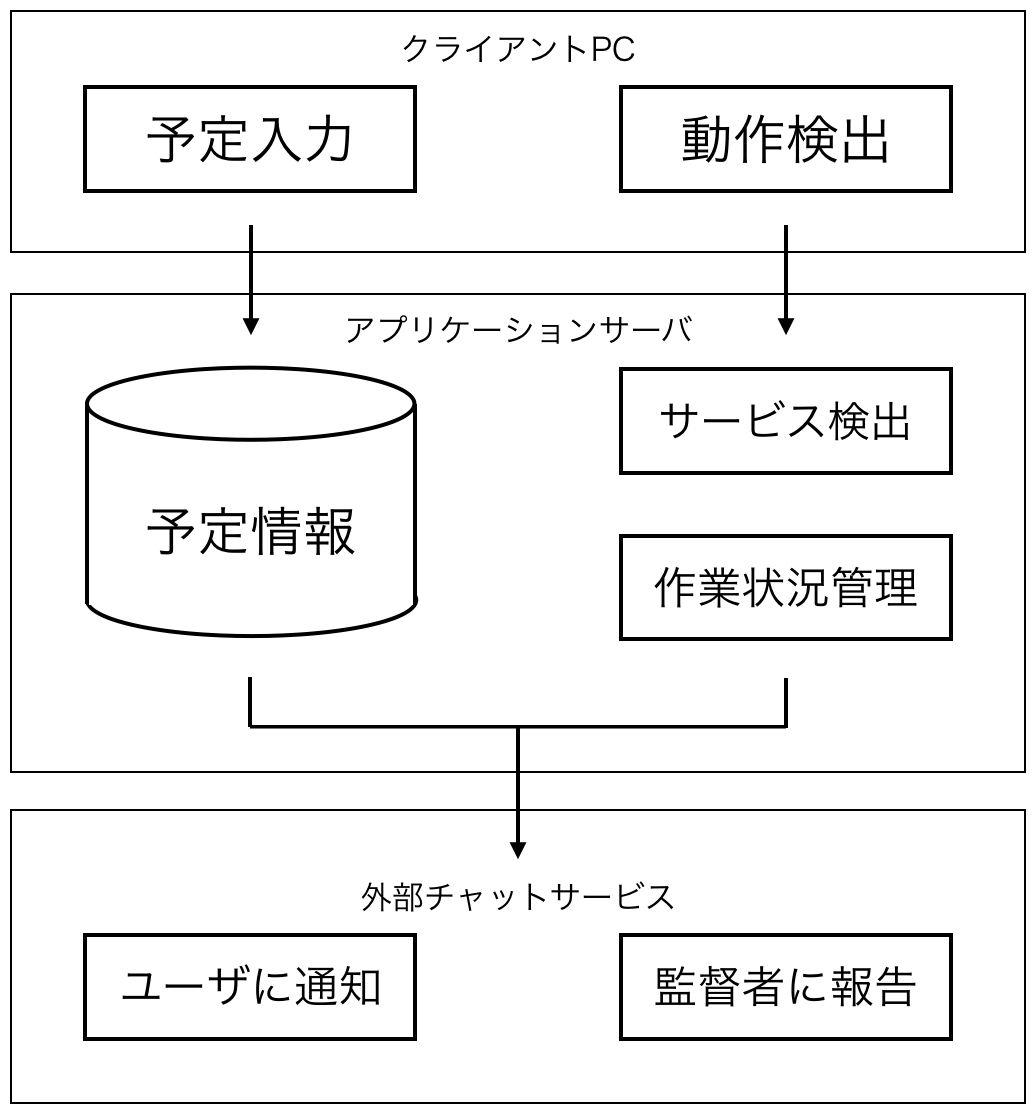
\includegraphics[width=9.0cm]{graphics/structure_chart.png}
  \caption{システム構成図}
  \label{fig:structure_chart}
  \end{center}
\end{figure}

\section{予定の管理機能}
ユーザは,システム利用開始時に,作業予定の設定を行う.設定内容は,作業内容と作業予定日時で構成される.
設定された作業予定は,ユーザへの通知や,監督者へ状況を報告する際に利用される.
また,作業全体の進捗状況は,設定された予定が基準になっている.
ユーザはアプリケーション内でいつでも予定を変更することが可能であるが,予定を変更した履歴も監督者に通知される.

\section{アプリケーションによる監視}
本システムでは,アプリケーション内でPCを監視する際,ユーザの作業状況の記録及び,利用中のサービスの検出を行う.

\subsection{作業状況の記録}
アプリケーションの起動状況は,ユーザがバックグラウンドで本システムを起動させておくことで,自動的にサーバに記録される.
また,作業予定になっているもののうち,現在何の作業を行っているのかをユーザが能動的に記録することも可能である.
ただし,自動検知された起動状況は,ユーザ自身が書き換えることはできない.

\subsection{サービス検出}
本研究でのアプリケーションでは,ユーザのPC上で現在表示している画面から,サービスの検出を行う.
まず,アプリケーションが起動している間,ユーザがPC上の画面をキャプチャ画像として自動的に保存する.
その後サーバ上で,それらの画像を解析することにより,ユーザが利用しているサービスの検出を行う.
画像の解析は,Google社のサービスである, Google Cloud Vision API (以下,Vision API)を利用する.

ユーザの画面キャプチャ画像を Vision API に通すことにより,その画像内に含まれるモノ,テキスト情報,サービスのロゴ画像等が検出される.
それらの情報を元に,ユーザが作業に不要なサービスを利用していないかの判別を行う.


\subsection{通知}
アプリケーションからユーザ及び監督者へ通知には,外部のチャットサービスを利用する.
まず,設定された作業予定時に,ユーザに対して通知が送信される.
ユーザは,チャットサービスから受け取る通知により,作業時間であることを認識できる.
また,1日に1回,決まった時刻に,前日の作業記録を監督者に通知する.
監督者は前日の作業記録を確認することにより,ユーザが作業を行った時間や,作業状況を把握することができる.

\clearpage

\section{作業記録の生成}
ユーザは,アプリケーション内で常に自分の作業状況を確認することができる.
作業記録は,主に2種類の形式で生成される.

1つは図\ref{fig:activity_table}のように,作業時間をテーブル上に色分けしたものである.
そのテーブルの上に,作業が行われた時間帯が色分けされる.
テーブルの色分けは以下のように設定した.

\begin{table}[h]
  \begin{tabular}{ll}
    カラーコード & 記録 \\
    ebedf0 & 作業予定時間外 \\
    eeff41 & 作業を行っていた \\
    f9fbe7 & 作業を中断していた \\
    3e2723 & 作業予定時間に,作業ができていなかった \\
  \end{tabular}
\end{table}

\begin{figure}[h]
  \begin{center}
  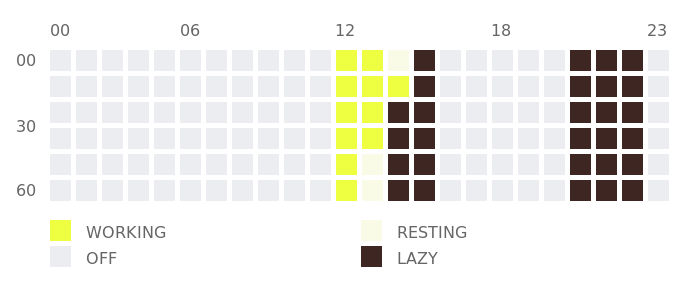
\includegraphics[width=12.0cm]{graphics/activity_table.png}
  \caption{作業時間のテーブル}
  \label{fig:activity_table}
  \end{center}
\end{figure}

\clearpage

2つ目は,ユーザのアプリケーション内の動作を記録した情報である.
図\ref{fig:activity_log}のように,動作の検出時間と,内容をリスト形式で表示する.
これらの作業記録はすべて監督者への通知でも利用される.

\begin{figure}[h]
  \begin{center}
  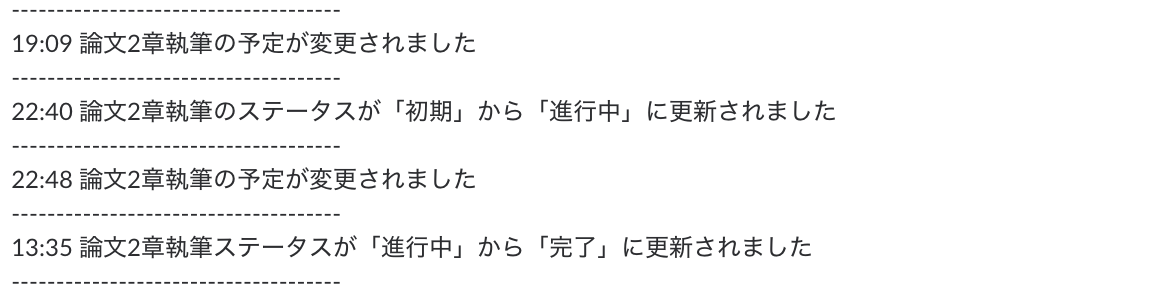
\includegraphics[width=14.0cm]{graphics/activity_log.png}
  \caption{作業時間のテーブル}
  \label{fig:activity_log}
  \end{center}
\end{figure}

%以降削除すること
\clearpage
\noindent
一二三四五六七八九零一二三四五六七八九零一二三四五六七八九零一二三四五\\
二\\
三\\
四\\
五\\
六\\
七\\
八\\
九\\
零\\
一\\
二\\
三\\
四\\
五\\
六\\
七\\
八\\
九\\
零  行数と列数の設定テスト 30行×35文字 = 1050文字/ページ\\
一\\
二\\
三\\
四\\
五\\
六\\
七\\
八\\
九\\
零

 % 3章
%\chapter{実験}
本章では,提案するシステムの有用性を検証する実験について述べる.

\section{目的}
この実験の目的は,ユーザと管理者両方の視点から有用性を測る.
まず,ユーザがシステムを利用することによって,作業の生産性が向上するかどうかを検証する.
また,管理者は,自動的に報告されるユーザの作業状況を確認し,現状を把握できるかどうかを確認する.

\section{対象}
実験は20代大学生9名と,研究室の指導教員1名を内訳とした10名対象とした.
実験は2017年11月3日から40日間実施した.

\subsection{対象者の定義}
学生は,作業の監視対象として,システムの利用者(ユーザ)である.
教員は,システムから作業状況の報告を受ける監督者である.

\subsection{作業の定義}
今回の実験では,研究室に所属する大学生の論文の執筆を監視する.
論文の執筆は,各個人のPCを利用し,文章作成用のソフトウェアを利用する.
したがって,文章作成用のソフトウェアを起動し,文字を入力することが今回の作業の定義とする.
その際,PCからインターネットを利用して情報を収集することも作業の範囲内とする.
ただし,アニメ動画やゲームなど,明らかに研究と関連しないものを閲覧する行為は作業の範囲外とする.

作業を検出する準備として,予め作業状態を表す情報を収集した.
まず,各個人が作業をしている際のPCの画面キャプチャ画像を50枚集め,解析を行った.
表\ref{tab:positive_words}は,解析によって得られた情報のうち,複数回出現したものである.

\begin{table}[htb]
  \begin{center}
    \label{tab:positive_words}
    \caption{複数回検出された情報}
    \begin{tabular}{lll}
      text & web page & website \\
      software & technology & product  \\
      black & computer program & Debian GNU/Linux \\
      font & screenshot & line \\
      black and white & &
    \end{tabular}
  \end{center}
\end{table}

画像キャプチャ解析において,これらに含まれる範囲の情報を検出した場合は,作業に必要な画面を表示していると判定する.
これら以外の情報を検出した場合は,作業範囲外であると判定する.

\section{実験手順}
監視対象であるユーザは,論文を執筆する際にアプリケーションを起動する.
本システムは,起動中のアプリケーションから収集される情報をもとに,作業記録の生成を行う.
生成された作業記録は,次の日の朝に,チャットサービスを通じて管理者に送信される.
それらの一連の流れを確認することで,システム自体の信頼性や情報の適正性を測る.

本システムに対するユーザ及び監督者の評価は,アンケート調査によって行う.
このアンケートでは,構築した監視システムの有用性や,実用的であるかどうかを調査する.

\section{結果}
本システムを2ヶ月間運用し,得られた結果を示す.
まず,監視システムによりユーザの論文執筆の作業を監視した結果を述べる.
その後,ユーザと監督者それぞれの視点から,本システムの評価を受けた結果を述べる.

\subsection{監視システムの運用}
本システムの運用は,作業予定の入力・監視・報告までユーザ及び監督者のみで行われる.
作業予定の入力を行うのはユーザのみであり,予定の追加や変更,削除など全て正常に動作した.
また,アプリケーションによる監視機能も自動的に行われ,PCからサーバへのデータの送受信も正確に行われた.

作業に不要なサービス・アプリケーションは,運用中に970回検出された.
検出されたのはAmazonやYahoo JapanなどのWebサービスや,SkypeやSlackなど,PC上で動作するアプリケーションであった.
他にも,ユーザのデスクトップに設定された画像なども作業範囲外の状態として検出された.

作業状況の報告は,午前中の時間帯に自動的に行われた.
作業をしていた時間帯,作業日時の変更,不正なサービスの検出など,システムで設定された項目は全て記録され,正常に送信された.
作業時間の通知機能も,事前に設定した作業予定時刻に従って正常に動作することが確認できた.

\subsection{ユーザによる本システムの評価}
作業を行う立場のユーザの視点から本システムを評価するためのアンケートは,監視対象であった9名ユーザを対象に実施した.
アンケートは,4段階評価で選択する形式と,自由に記述する形式の2種類で回答する.
各質問項目と,回答状況から,本システムに対する評価を述べる.

\subsubsection{本システムにより作業をやらないといけない気になったか}
9名全員が「なった」あるいは「少しなった」と回答した.
本システムにより,作業を行う動機付けが可能であり,行動を促すことを期待できることが分かった.

\subsubsection{本システムを使うことによって生産性は向上すると思うか}
9名全員が「とても思う」あるいは「思う」と回答した.
本システムを利用することによって,作業者の生産性の向上が期待できるという評価がされた.

\subsubsection{自身の作業が報告されることに抵抗があるか}
7名が「抵抗がある」と回答し,2名が「あまり抵抗がない」と回答した.
このことから,作業が監視されることに抵抗を感じるユーザは少なくないと考えられる.
監視システムを構築する上で,監視対象であるユーザの抵抗感をなくしていくことが今後の課題として挙げられる.

\subsubsection{作業を行う際,本システムに監視されていることを意識したか}
7名が「とても意識した」あるいは「意識した」と回答し,2名が「あまり意識していない」と回答した.
意識するユーザが多かったことから,システムにより,作業を開始する際だけでなく,作業中も影響をあたえられることが分かった.

\subsubsection{予定を管理するにあたって,本システムは使いやすいと思うか}
1名が「使いやすい」と回答し,8名が「やや使いにくい」と回答した.
今回のシステムでは,作業内容と日時を入力する簡素な構造であったため,正しく予定を管理するためには,個人が管理するカレンダーと連動させるなど,工夫しなければならない.
また,スマホで管理できるようにしてほしいなど,より手軽さを求める意見も見られた.

\subsubsection{作業開始時間の通知は役に立ったか}
7名が「役に立った」と回答し,2名が「あまり役に立たなかった」と回答した.
「あまり役に立たなかった」と回答した理由として,「通知を確認しても,その時点でのモチベーションが低かったため,行動に移せなかった」という意見が得られた.
したがって,通知により開始時間を認識させることはできていたが,それにより実際に行動を促すということについては,さらなる工夫が必要である.

\subsubsection{通知の頻度は適切であったか}
3名が「適切である」と回答し,6名が「多い」あるいは「とても多い」と回答した.
今回は作業時間から30分毎に繰り返し通知を行うように設定を行ったが,頻度が多い感じたユーザが多く見られた.
ただし,作業の開始を促すための通知であるため,多いと感じる程度が適切であると考える.

\subsubsection{システムによって進捗管理を自動化することは現実的だと思うか}
8名が「現実的である」と回答し,1名が「現実的ではない」と回答した.
「現実的である」と回答した人の意見として,「利用してみて可能だと考えた」というものや,「進捗管理は人間よりもシステムがやったほうが効率的である」というものが挙げられた.
それに対し「非現実的である」と回答した人の意見としては,「プライバシーの面で実現が難しいのではないか」というものが挙げられた.

\subsubsection{その他,システムに関する意見}
本システムを利用することによって,「やらないといけないという気持ちになった」という意見が複数あった.
他にも実績が可視化されることがモチベーションにつながるなど,報告される情報そのものに価値を感じているユーザも見られた.
また,「オフライン環境で動作することができない」「予定の入力が大変である」といった意見もあり,システム自体をより手軽なものにしてほしいという要望が寄せられた.

\subsection{監督者による本システムの評価}
監督者の立場から本システムを評価するためのアンケートは,実際に本システムを利用してユーザを監督した1名の教員を対象に行った.
以下はアンケートの各質問項目と,その回答である.

\subsubsection{本システムにおいて有効だった点}
実際に作業している時間がわかることによって,あとどれぐらいの時間やるべきなのかを具体的に指導することができた.

\subsubsection{本システムにおいて不足していた点}
動かしていない場合などの記録が得られないこと.
作業をする予定で何もいない場合と,作業をする予定で別のことをしている場合の区別ができないように思える.
また,作業をしない予定で作業をしていない場合も区別出来た方が,より具体的な管理につながると考えられる.

\subsubsection{システムによって進捗管理を自動化することは現実的だと思うか}
職場での利用を考えると現実的であるが,学生の実態では非現実的かと思われる.
職場では業務時間内に他の個人的なことや連絡にPCを利用することはないが,学生個人のPCでは作業をしながら別の個人的なことを行うのが一般的と想定できるためである.
ただし,学生にも集中して作業する時間を確保するように十分な指導ができれば,現実的であると考えられる.

\subsubsection{その他,システムに関する意見}
本システムを学生に利用してもらってわかったのは,個人で進捗管理ができていないことである.
具体的には,多くの学生は,タスクの詳細化とそれを消化する時間の設定,週や日ごとの消化しきれなかったタスクの見積もりと再配置ができていない.
現状のシステムでも可能だが,そもそもTODO管理が出来ないために,有効活用できていない.
管理ユーザーとしては,管理者ユーザ側が各自のタスクとタスク詳細化と時間の見積もりに関与し,それを各自に割りふりさせ,状況を確認するようなシステムにした方が,より確実に進捗管理が可能となる.

一方,管理ユーザの手を煩わせること無く,管理ユーザに通知されていることを意識することによるなまけ抑止を期待するのであれば,システムは現状のままでも十分である.ただし,前述の通り現状のタスク消化・作業実施状況から,利用ユーザはTODO管理のコツが理解できておらず,最低限そのレクチャーを行う必要がある.

\section{考察}
本システムについて,有用性を検証するために行った実験の考察を述べる.
進捗監視を行うにあたって,実際にユーザが作成した予定を元に作業時間を記録し,自動的に報告を行うことができた.
これにより,ユーザが作業を行う動機付けがなされ,行動を促すことができた.
また,報告される情報により,監督者の立場から,より具体的に作業者に指導を行うことが可能となった.
以上のことより,本システムの有用性が高いことが検証された.
 % 4章
%\chapter{おわりに}
本章では,本研究のまとめを論述する.また,今後の課題について述べる.

\section{まとめ}
本研究では,個人のPCワークの進捗管理により,生産性を向上させることを目標としたシステムを構築した.
実験では実際にシステムの運用を行い,利用者からの評価を受け,提案したシステムの有用性を測った.

システムの運用を行なった結果,ユーザが作成した予定を元に作業時間を記録し,自動的に報告を行うことができた.
これにより,ユーザが自身の作業を行うように促す効果があることも判明した.
また,報告される情報も,監督者も作業者の現状を確認し,指導に役立つものであると評価された.
以上のことより,本システムの有用性が高いことが検証された.

\section{今後の課題}
本研究で構築したシステムの問題点は,個人の予定を正しくシステムに反映させることが難しいことである.

システムで正確な予定管理を実現することができなかった原因として,予定管理の入力に手間がかかることが挙げられる.
本研究では,構築したアプリケーション内で各個人の予定の入力がそれぞれで行われた.
この方法はユーザがシステムを能動的に利用し,個人が自ら予定を管理しなければならない.
ユーザが予定管理を自身で行うことができなかった場合,監督者も作業者の現状を正しく認識することができない.
管理される予定の精度を高めるためには,予定の入力によるユーザの負担を軽減し,手軽に利用できるシステムにしなければならない.
あるいは,ある程度,監督者が作業内容や作業時間を見積もり,ユーザはそれを各自の予定に割り振るような形式にすることで,より確実に予定の管理が行われると考える.

進捗監視システムをより現実的なものにするためには,より正確な予定の管理機能を実現することが重要である.
そのためには,信頼性が高く,ユーザにとってより使いやすいシステムにしていく必要がある.
また,組織で運用していく中で,システムを通じてコミュニケーションがとれるサービスとして進化させていくことにより,組織全体の生産性を向上させるものになると考える.
 % 5章
%\include{chap6} % 6章
\end{verbatim}
}
\end{breakbox}

なお,これらのファイルは通常の\verb+\chapter+など \LaTeX の命令でマークアップしていけば良い.
chapter1.tex や chapter2.tex,chapter3.tex 内を見れば,おおよその方法は理解できるはずである.

\subsubsection{付録の設定と読み込み}
付録は以下の様になっている.
\begin{breakbox}
{\small
%footnotesize
\begin{verbatim}
%%% 付録 -- 必要なければ以下を2行コメントアウト
\appendix
\chapter{プログラムの動作方法}
本研究にて用いたプログラムについて解説する.

\section{ファイル構成}
プログラムのフォルダ内は,主に4つのファイルから構成される.

ああああいいいい

ううううええええ

これらを○○に設置し,以下の手順にそって起動する.

\section{起動方法}
まず,ウェブサーバを動かした状態にし,外部クライアント(Webブラウザから),以下のURLにアクセスする.


\section{表示の見方}
実験に利用するための,実行結果は test.log ファイルに出力されている.

このファイルは4つのカラムからなる CSV形式のファイルである.
第1列には,…





%\include{appendixB} %必要に応じて付録の数を増やす
\end{verbatim}
}
\end{breakbox}
サンプルとして 付録A(appendixA.tex)だけ読み込む様にしている.
このファイルも通常の\verb+\chapter+など通常の\LaTeX の命令でマークアップしていけば良い.
また,必要に応じて追加,コメントアウトして構わない.

\subsubsection{参考文献の設定と読み込み}
最後に参考文献の設定がなされている.
\begin{breakbox}
{\small
%footnotesize
\begin{verbatim}
\bibliographystyle{junsrt}
\bibliography{myrefs}
\end{verbatim}
}
\end{breakbox}
\verb+\bibliography{myrefs}+によって myrefs.bib ファイルが読み込まれている.
このファイルは \BibTeX のフォーマットにて記載されている.
詳細は3章にて記述する.
